\documentclass[smallextended]{svjour3}
\smartqed%
\usepackage{simplemargins}
\usepackage{url}
\usepackage{graphicx}
\usepackage{setspace}
\usepackage{siunitx}
\setallmargins{1in}
\usepackage{natbib}
\usepackage{color}
\usepackage{subfigure}
\usepackage{booktabs}
\usepackage{pdflscape}
\usepackage[colorlinks=false,breaklinks]{hyperref}
\usepackage{lineno}
\usepackage{longtable}
\linenumbers%
\listfiles%

% make subfigure labels capitalized
\renewcommand{\thesubfigure}{(\Alph{subfigure})}

%setup supplement
\newcommand{\beginsupplement}{%
        \setcounter{table}{0}
        \renewcommand{\thetable}{S\arabic{table}}
        \setcounter{figure}{0}
        \renewcommand{\thefigure}{S\arabic{figure}}
        \renewcommand{\thesection}{S\arabic{section}}
        \renewcommand{\thesubsection}{S\arabic{subsection}}
     }

%set citation punctuation according to website guidelines
\bibpunct[;]{(}{)}{;}{a}{}{,}%

\RequirePackage{fix-cm}

\begin{document}

\doublespace%

\title{The ecological genomics of gypsy moth invasion along a latitudinal
gradient}

\titlerunning{Gypsy moth invasion}

\author{Christopher J.\ Friedline \and
Trevor M.\ Faske \and
Erin M.\ Hobson \and
Brandon M.\ Lind \and
Dylan Parry \and
Rodney J.\ Dyer \and
Derek M.\ Johnson \and
Lily M.\ Thompson \and
Kristine L.\ Grayson \and
Andrew J.\ Eckert*
}

\institute{C.\ Friedline \at%
Department of Biology,  Virginia Commonwealth University, Richmond, VA  23284,
\email{cfriedline@vcu.edu}
\and
T.\ Faske \at%
Department of Biology, Virginia Commonwealth University, Richmond, VA  23284,
\email{fasket@vcu.edu}
\and
E.\ Hobson \at%
Department of Biology, Virginia Commonwealth University, Richmond, VA  23284,
\email{hobsonem@vcu.edu}
\and
B.\ Lind \at%
Department of Biology, Virginia Commonwealth University, Richmond, VA  23284,
\email{lindb@vcu.edu}
\and
D.\ Parry \at%
Environmental and Forest Biology, State University of New York, Syracuse, NY,
\email{dparry@esf.edu}
\and
R.\ Dyer \at%
Department of Biology, Virginia Commonwealth University, Richmond, VA  23284,
\email{rjdyer@vcu.edu}
\and
D.\ Johsson \at%
Department of Biology, Virginia Commonwealth University, Richmond, VA  23284,
\email{dmjohnson@vcu.edu}
\and
L.\ Thompson \at%
Department of Biology, University of Richmond, Richmond, VA  23173,
\email{lthomps2@richmond.edu}
\and
K.\ Grayson \at%
Department of Biology, University of Richmond, Richmond, VA  23173,
\email{kgrayson@richmond.edu}
\and
A.\ Eckert (*Corresponding author) \at%
Department of Biology, Virginia Commonwealth University, Richmond, VA  23284,
\email{aeckert2@vcu.edu}
}

\date{Received: date / Accepted: date}


% \author[1]{Christopher J. Friedline}
% \author[1]{Trevor M. Faske}
% \author[1]{Erin M. Hobson}
% \author[2]{Dylan Parry}
% \author[1]{Derek M. Johnson}
% \author[3]{Lily M. Thompson}
% \author[3,*]{Kristine L. Grayson}
% \author[1,*,\textdagger]{Andrew J. Eckert}
% \affil[1]{Department of Biology, Virginia Commonwealth University}
% \affil[2]{College of Environmental Science and Forestry, State University of
% New York}
% \affil[3]{Department of Biology, University of Richmond}
% \affil[*]{Authors contributed equally}
% \affil[ \textdagger]{Corresponding author}


\maketitle


\begin{abstract}
TODO

\keywords{}

\end{abstract}


\thispagestyle{empty}

\linenumbers%

\section*{Introduction}


Phenotypic and genetic differentiation of populations after establishment and
range expansion of an invasive species presents a novel opportunity to test
hypotheses regarding the process of local adaptation and the resulting genetic
structure of populations expanding across environmental gradients. Newly
established species face many challenges in order to succeed in
ecological conditions that may differ drastically from their native environment
and location of introduction. Adjustment in phenotypic traits, whether through
evolutionary mechanisms or plasticity, are vital to dispersal and early range
expansion. These processes rely heavily on prior evolutionary history and the
reaction norm of plasticity, as well as both deterministic and stochastic
events. [KG: DID I ADD TOO MUCH TEXT ON PLASTICITY?]

Demographic processes associated with invasions have been shown to limit
adaptive potential and negatively affect fitness landscapes. These events
include founder effects, genetic drift, population bottlenecks, and inbreeding
[CITE].  Invasive species are particularly susceptible to reductions in allelic
richness and heterozygosity due to these limiting processes. [KG: WHAT WAS
INTENDED BY ``and also varying selective regimes'' I DIDN'T WANT TO DELETE AND
LOSE THE INTENTION OF THE SENTENCE]  The key to divulging the underlying
mechanisms that change the genetic basis of fitness-related traits is to design
experiments that directly test selection and local adaptation [STENGTHEN THIS
SENTENCE, IT IS A BIT CIRCULAR].

Classical approaches in quantitative genetics TO TEST XXX include common garden
and reciprocal transplant experiments. Such designs inform the genetic basis of
selection and local adaptation by estimating fitness over an environmental
gradient but are limited in non-model, non-plant organisms due to the
feasibility of rearing natural populations in their natural environments over
multiple generations while keeping track of population pedigrees (Salvonian et
al.2013, Hirschhorn/Daly 2005). Often, the traits linked to fitness are
polygenic and identification of the genomic loci for these traits was nearly
impossible until recent advancements in sequencing technologies. Coupling new
genomic resources with classical approaches has vastly increased the inferential
power of detecting polygenic adaptation. Reduced sequencing costs have also made
genome-wide association studies (GWAS) possible for a large number of
individuals and organisms in natural populations not previously possible. [FOR
THIS AUDIENCE DO WE NEED TO INTRODUCE GWAS IN MORE DETAIL?]

^^Maybe split this into two paragraphs and talk about Fst outliers and linkage
disequilibrium before GWAS

When trying to equate phenotypic divergence of a trait among populations to
genomic regions, many studies will expect the same pattern of high divergence
within the genome. This analysis is usually performed by looking for Fst
outliers, but there have been many cases of discordance between levels of
differentiation among traits and their underlying loci (McKay/Latta2002).  High
levels of phenotypic divergence can be observed with little to no
differentiation within the genomic regions controlling these traits; thus making
them undetectable in Fst outlier based studies (LeCorre and Kremer 2003).
Conversely, in instances where there is little apparent phenotypic divergence in
populations, there can be important variation in genetic structure that provides
insights to the process of adaptive differentiation. Since polygenic traits are
affected by multiple loci, the detection of selection is spread out over loci so
a single locus can appear to be neutral or nearly neutral. Thus, non-detection
of selection at early stages could be evident at a single locus but there is
expected to be strong correlations in allelic effects. This creates large
covariances in allele frequencies of loci in the polygenic trait that becomes
the main driver of Qst and when a trait is under divergent selection, Qst > Fst
is expected of the underlying loci. (All Qst>=<Fst Papers, Kremer/LeCorre2012)

In this study, we used the North American invasion of the European gypsy moth as
a model to examine the genomic architecture of life history traits in
populations across the latitudinal extent of the invasive range.  Using a GWAS
approach to identify loci associated with phenotypic variation, we assessed the
differentiation of populations along this extent in terms of biologically
consequential traits. GWAS has strong inferential capabilities where we could
use associated SNP data to estimate multilocus parameters of heritability, Fst,
Qst, and linkage disequilibrium through (Bayesian mumbo jumbo).

\subsection*{Study System}

The European gypsy moth (\textit{Lymantria dispar dispar} L.) was introduced to
the United States in 1869 when individuals escaped from the collection of an
amateur naturalists and silk producer, Étienne Léopold Trouvelot, in Medford,
Massachusetts (Liebhold et al. 1989). While supplemental introductions have
likely occurred over the last 150 years, microsatellite analyses point to this
source as the main origin (Bogdanowicz et al. 1997). The severe bottleneck
surrounding the introduction of the species has led to the conclusion that
little genetic variation exists in gypsy moth population across North America
(Wu et al. 2015).

Notes from AJE: This was not shown by Wu et al. (2015). In fact, European
populations were about as diverse as NA populations (actually statistically  the
same). There was a slight numerical decrease in things like effective number of
alleles, but it was marginal and not significant.  This then implies that a
severe bottleneck either did not happen OR population growth has resulted in a
restoration of diversity. The latter is likely given that private alleles were
noticed in the EXPANDING AND GROWING populations on the range edge.  Wu et al.
(2015) did talk a lot about their belief in a bottleneck and their feelings
about it, but based on my reading did in no way demonstrate one, unless they are
referring to both European and NA populations relative to Asian populations. A
quick inspection of their data tables reveals that heterozygosity is still quite
high and almost numerically equal to Europe.

However, the current gypsy moth invasion front spans north into Canada, west
into Minnesota, and as far south as North Carolina, and populations are
experiencing very different selective pressures across this range based on
climate and community composition. The combination of its wide geographic range,
its known point of introduction, and its extremely well-documented spatial
spread (Tobin et al. 2007) makes the North American gypsy moth an ideal model
for examining the genetic architecture of an invasive species.

Gypsy moths have a univoltine life cycle where caterpillar larvae hatch, grow
until pupation, and emerge as adult moths in the spring and summer, laying eggs
that overwinter in diapause. Hatch is generally timed with budburst of their
preferred hosts, oak and aspen; however the gypsy moth is a generalist herbivore
that will feed on more than 300 foliage hosts as larvae (Liebhold et al. 1995).
Adults live between x and x days and do not feed during this time. Adult female
\textit{L. dispar} are flightless and release pheromones to attract flying male
mates (Doane and McManus 1981). Given the small window of opportunity to mate
each year, the success of a gypsy moth population depends on the overlap of adult
emergence between males and females (reference). Latitudinal variation in
developmental timing traits can impact this overlap, as well as the synchrony
for larval developmental with preferred host trees.

The well-developed pheromone signaling system of the gypsy moth has been
exploited by forest pest managers for decades as an assessment tool for trapping
regimes to measure spread and abundance. Pheromone-based solutions have also
been developed for management through the development of mating disruption
treatments. These efforts specifically target male gypsy moths and the extensive
data assessing the progression of the North American invasion front is based
exclusively on male moth captures, as females are flightless and not detectable
at the same spatial scale. Therefore, we focus our analysis on traits in male
gypsy moths to maximize the utility of our results to researchers and forest
managers.

In many insect species, including the gypsy moth, larger individuals have higher
fecundity. In the gypsy moth, growth occurs entirely in the larval stage and
climaxes just prior to pupation. A frequent measure of fitness for the gypsy
moth is pupal mass, as this traits both represents growth during larval
development as well as egg characteristics in females (reference).In gypsy moth
females, as in other insects, size is directly related to egg load, with larger
females producing more eggs. Thus, larger females are considered more fecund
than smaller females. Although we examining phenotypes of male moths in this
study, the larval conditions that produce larger individuals do so for both
males and females. Size advantages specifically for males include increased
flight capabilities and longer survival duration as an adult to find potential
mates.


\section*{Methods}

\subsection*{Sampling}

(State where climate data came from here)

\subsection*{Phenotype determination}

\subsection*{Library preparation and sequencing}

Genomic DNA extracted using Qiagen DNeasy Blood and Tissue kits (Qiagen, cat \# 69581)
according to manufacturer's protocol.  The library was prepared and sequenced as
a single run of paired-end reads on the Illumina HiSeq 2500 platform at the
Virginia Commonwealth University Nucleic Acids Research Facility. Quality was
initially assessed using FastQC \citep{fastqc} and subsequently processed with
IPython \citep{Perez:2007hy} and BioPython \citep{Cock:2009hj}. The read pairs
were each evaluated along sliding windows of 5 base pairs (bp).  If the mean
score in this window was below a score of 30, the read was trimmed at that
beginning of the window. If the shortened read was less than 50\% of the length
of the original read, it was discarded along with its pair. Additionally, if
20\% of the bases in a read had quality values less than 30, it was discarded
along with its pair.

\subsection*{Draft assembly}

An assembly was produced for the purpose of variant calling and is not
considered as a candidate for complete genomic assembly. The quality-filtered
reads from the paired-end sequencing library was used as input into
\texttt{MaSuRCA} \citep[][versions 2.3.2, 3.1.3]{Zimin:2013kn}, with the
following parameters changed from the defaults: mean/standard deviation of read
length: 400/60, use linking mates: 1: cgwErrorRate: 0.15.  Quality of the
assembly was assessed using the statistics generated by the assembly process, as
well as with the \texttt{BUSCO} \citep[][version 1.1b1]{Simao:2015kk} and
\texttt{QUAST} \citep[][version 3.2]{Gurevich:2013je}. For \texttt{BUSCO}, the
software was built automatically using a Docker image (see GitHub repository
information below). The assembly was evaluated against pre-computed
\texttt{Augustus} \citep{Stanke:2003eo} metaparameters of three species
(\textit{Aedes}, \textit{Heliconius}, and \textit{Drosophila}) and the BUSCO
Arthropoda lineage profile using a \texttt{tblastn} e-value cutoff of $0.001$.
For \texttt{QUAST}, the software was executed using the following options
(\texttt{--gene-finding, --eukaryote, --glimmer, --min-contig 200}).  Results
from both \texttt{BUSCO} and \texttt{QUAST} were used to determine which
assembly to use for downstream analysis.

The assembly as aligned using BLASTX \citep[][version 2.2.30+]{Camacho:2009fc}
to genes from \textit{Bombyx mori} (June 2, 2015) and  \textit{Plutella
xylostella} (March 13, 2015), keeping at most five target sequences from each
geneme with alignments having e-values less than $10^{-5}$.


\subsection*{Sequence processing and variant calling} Sequencing of 170
individual moths, exclusive of the one used for assembly,  as performed on
reduced genomic DNA per~\cite{PARCHMAN:2012ca}. In total, two Illumina HiSeq
2500 lanes were sequenced. Bases with quality scores less than 33 were masked,
per~\cite{Yun:2014dn},  using \texttt{fastq\_masker} from the FastX toolkit
\citep[][version 0.0.14]{citeulike:9103573}.

Masked fastq files were mapped using \texttt{bowtie2}~\citep[][version
2.2.4]{Langmead:2012jh}, using flags  \texttt{--local --very-sensitive-local}.
The resulting  SAM files were converted to their binary equivalent, sorted,
and indexed. To each of these indexed bam files, appropriate \texttt{RG} ID and
sample information was added using \texttt{Picard}
(\url{https://broadinstitute.github.io/picard}), version 1.112 to inform variant
calling.

Sequence variants were called using samtools and bcftools \citep[][version
1.3]{Li:2009ka} with individual  ploidy level set to \texttt{2} for all samples.
The variants were filtered  using \texttt{vcftools}~\citep[][version
0.1.14]{Danecek:2011gz}, such that only biallelic single nucleotide
polymorphisms (SNPs) remained in cases where a variant call was present in at
least 50\% of the samples and the minimum genotype quality (\texttt{--minQG}) of
3. An additional filtering using \texttt{vcfutils.pl} (from \texttt{bcftools})
was performed to only keep sites with mapping qualities of at least 10
(\texttt{varFilter -Q 10}). The vcf file was then double checked to ensure all
reference and alternate alleles were single nucleotides before imputation with
\texttt{Beagle} \citep[][version 4.0, r1399]{Browning:2007ge}.  The imputation
was performed on 30 CPUs using the following non-default parameters:
\texttt{phase-its=20, burnin-its=20, impute-its=20}.

For each set of imputed (IMP) and non-imputed (NI) SNPs, the following filtering
was performed.  First, \texttt{VCFtools} was used to include only biallelic
SNPs (\texttt{--min-alleles=2, --max-alleles=2}), SNPs with minor allele
frequency (MAF) of at least 1\% (\texttt{--mac=0.01}) and SNPs present in at
least 50\% of the samples (\texttt{--max-missing=0.5}).  Additional MAF
(correcting for  finite population size) and percent missing filtering was done
using Python following removal of duplicate samples from the variant data and
depth across samples (DP), Alternate allele call quality (QUAL), and RMS mapping
quality values (MQ), reported in the VCF file were examined.  An additional
filtering step was conducted using \texttt{vcfutils.pl} (from \texttt{bcftools})
to remove SNPs with MQ values less than 10.  Monomorphic SNPs were removed as
well as SNPs with $F < -0.5$ or $F > 0.5$.  We only considered SNPs
to be valid if they passed filtering in both the IMP and NI datasets. Finally,
SNPs were oriented according to dosage of globally-minor allele, rather than
alternate allele with respect to the assembly. In other words, in a file of
genotypes where 0/1/2 would normally represent counts of alternate allele in a
diploid genotype,  (as output by \texttt{VCFtools}), 0/1/2 were recoded to
represent counts of the minor allele (i.e., a genotype of 2 indicates two copies
of the globally minor allele). This ``swapped'' representation was then used as
input for downstream analysis.

\subsection*{Patterns of phenotypic and genetic variation}

Values for each phenotypic trait were summarized  within populations using
parametric summary statistics (i.e., means and variances). Differentiation among
populations for phenotypic traits was assessed using Multivariate Analysis of
Variance (MANOVA). Statistical significance of the MANOVA model was determined
using Wilk's lambda as the test statistic and $\alpha = 0.05$. We subsequently
used one-way Analysis of Variance (ANOVA) to assess differentiation separately
for each phenotypic trait. We treated population identifiers as a fixed effect
for statistical hypothesis testing ($\alpha = 0.05$), but as a random effect for
estimation of variance components. Variance components were used to construct a
measure of phenotypic differentiation akin to hierarchical $F$-statistics.
Specifically, we used the ratio of the variance due to population identifiers to
the total phenotypic variance ($P_{ST}$) as a measure of phenotypic
differentiation. Parametric bootstrapping ($n = 1000$ replicates) was used
to derive confidence intervals around point estimates of $P_{ST}$. All analysis
was conducted using the \texttt{stats} and
\texttt{lme4} libraries of R ver. 3.1.2 (R Core Team 2014).

Patterns of genetic variation within and among populations were described using
standard population genetic indices: observed ($H_{obs}$) and expected
($H_{exp}$) heterozygosities, Wright's inbreeding coefficient ($F$), and
hierarchical $F$-statistics (e.g. $F_{ST}$). Estimates were made for each SNP
and all SNPs combined using the \texttt{hierfstat} library in R. Confidence
intervals ($95\%$) for multilocus estimates were generated using bootstrapping
across SNPs ($n = 1,000$). Genetic structure among populations was also assessed
using principal components analysis (PCA) following~\cite{Patterson:2006}.
Significance of principal components (PCs) was determined using Tracy-Widom
tests with $\alpha = 0.05$ \citep{Patterson:2006}.

Lastly, we used redundancy analysis (RDA) to describe the effects of climate,
genetics, and geography on phenotypic trait values. We partitioned the variance
using standard variation partitioning methods \citep{Borcard:1992, Liu:1997}.
Geography was quantified using latitude and longitude, with both measures
centered and standardized prior to analysis, while climate and genetics were
quantified using PCs derived from PCA. For climate data, PCs with eigenvalues
$> 1$ were retained for further analysis. For genetic data, PCs that were
associated with statistically significant eigenvalues, as assessed using
Tracy-Widom tests, were retained for further analysis. All PCs were
centered and standardized prior to analysis. Statistical significance
of RDA models, as well as RDA axes within these models, was tested using
a permutation-based ANOVA with $9,999$ permutations \citep{Legendre:2011}. All
RDA analyses were performed using the \texttt{vegan} library in R. 


\subsection*{Genome-wide association analyses}

Correlations between allele frequencies and environmental variables were
evaluated using \texttt{Bayenv} \citep[][version
2.0]{Gunther:2013ik,COOP:2010ke}. Bayes factors and correlation coefficients
were evaluated for each SNP using \num{100000} MCMC iterations.  The covariance
structure among populations was obtained from final variance-covariance matrix
output, sampled every 500 steps over \num{100000} iterations.  MCMC convergence
was assessed by sequential matrix-matrix correlations.

Genotype-phenotype correlations were investigated using Bayesian Sparse Linear Mixed
Models (BSLMMs) implemented in \texttt{GEMMA} \citep[][version
0.94.1]{Zhou:2013fh}.  Effects of  genotypes on phenotypes, after correcting for
population structure with PCA and normal-quantile transformation, were evaluated
across four separate MCMC chains of \num{100000000} generations, sampled  every
1000 steps.  Convergence was evaluated using the \texttt{coda} package in R
\citep[][version 0.18.1]{coda} using, effective sample size ($> 100$) estimates,
trace plots and visual examination of the posterior distributions. Posterior
effect estimates for each SNP were estimated as the harmonic mean of values
across each chain.


\subsection*{Genetic architecture and selection}
TODO

\section*{Results}

\subsection*{Draft assembly and DNA sequence analysis}
TODO

\subsection*{Patterns of phenotypic and genetic variation} Average phenotypic
trait values were correlated across populations, with mass strongly correlated
with pupal duration time (Pearson's $r = 0.804$) and total development time
(Pearson's $r = 0.782$).  Neither of these correlations, however, were
statistically significant at $\alpha = 0.05$. Phenotypic trait values also
varied across populations, with population labels statistically differentiating
multivariate trait values (MANOVA: Wilk's $\lambda = 0.663, F_{5,164} = 4.798,P =
1.149$e-$08$). Inspection of results from one-way ANOVAs revealed that this
effect was driven largely by total development time (ANOVA: $F_{5,164} = 8.354,P =
4.658$e-$07$), with mass marginally differentiated among populations (ANOVA:
$F_{5,164} = 3.120,P = 0.010$). No effect was apparent for pupal development
time. These results were consistent with point estimates for $P_{ST}$, where
population labels accounted for $22.88\%$ ($95\%$ CI: $1.18 - 46.48\%$) of the
variance for total development time and only $7.07\%$ ($95\%$ CI: $0.00 -
20.13\%$) of the variance for mass.

<Chris: brief summary about genetic PCA and FST here, for example PC1 is
+correlated with lat and long. PC2 is -correlated with long. Also, you should
look for correlations of lat and long with obs and exp heterozygosity within
pops. Also state similarity between PCA with NI and IMP.>

Phenotypic trait values were significantly correlated with geography, climate,
and genetic variation (RDA: $F_{19,150} = 2.369, P = 1.0$e-$04, R^2 = 0.231$;
Figure 2). All three RDA axes were statistically significant ($P < 0.001$). 
The first two RDA axes explained $86.60\%$ of the total
explainable variation (i.e. $86.60\%$ of $R^2 = 0.231$). These two axes were
dominated by mass and total development time, with the first axis reflecting the
correlation between mass and total development time and the second axis
differentiating these two traits. The remainder of the explainable variation was
attributed to third axis, which was dominated by pupal duration time. The first
RDA axis was highly correlated with environmental PC 1, genetic PCs 1 through 3,
latitude, and longitude, whereas the second RDA axis was most correlated with
environmental PC1, genetic PCs 4 and above, and latitude (Figure 2).

Partitioning the contribution of each type of explanatory variable to the overall
explanrevealed that
genetic variation and geography had the largest pure effects on phenotypic trait
variation (Figure 2B). Of these, genetic PCs accounted for the vast majority
(i.e. $68.74\%$) of the total effect. Testing the statistical significance of
the partial RDA (pRDA) models used to estimate pure effects of each variable was
consistent with the magnitudes of explanatory power. The pRDA models for genetic
variation conditional on geography and climate and geography conditional on
genetic variation and climate were both statistically significant ($P < 0.006,
R^2 > 0.035$), whereas the model for climate conditional on genetic variation
and geography was not ($F_{2,150} = 1.384, P = 0.223, R^2 = 0.014$). The effects
of climate on phenotypic trait variation were thus small and confounded with
either genetic variation ($4.72\%$) or geography ($3.08\%$).


\subsection*{Genome-wide association analyses}
TODO

\subsection*{Genetic architecture and selection}
TODO

\section*{Discussion}
TODO


\section*{Conclusion}
TODO


\begin{acknowledgements} The authors would like to thank the staff at
the VCU Nucleic Acids Research Facility and the
VCU Center for High Performance Computing.  CJF was supported by the National
Science Foundation (NSF) National Plant Genome Initiative (NPGI): Postdoctoral
Research Fellowship in Biology (PRFB) FY 2013 Award \#NSF-NPGI-PRFB-1306622.
(CJF - Need more from Kristine and Andrew)
\end{acknowledgements}

\section*{Data Archiving Statement}

Raw short read data are located in the NCBI Short Read Archive (accession
number: XXXXX). Source code for the data analysis and this manuscript are
located at
\url{http://www.github.com/cfriedline/gpysy_moth} and \url{/gypsy_moth_ms},
respectively.

\clearpage
\bibliographystyle{spbasic}
\bibliography{refs}

\clearpage


\section*{Figures}
\begin{figure}[ht]
\centering
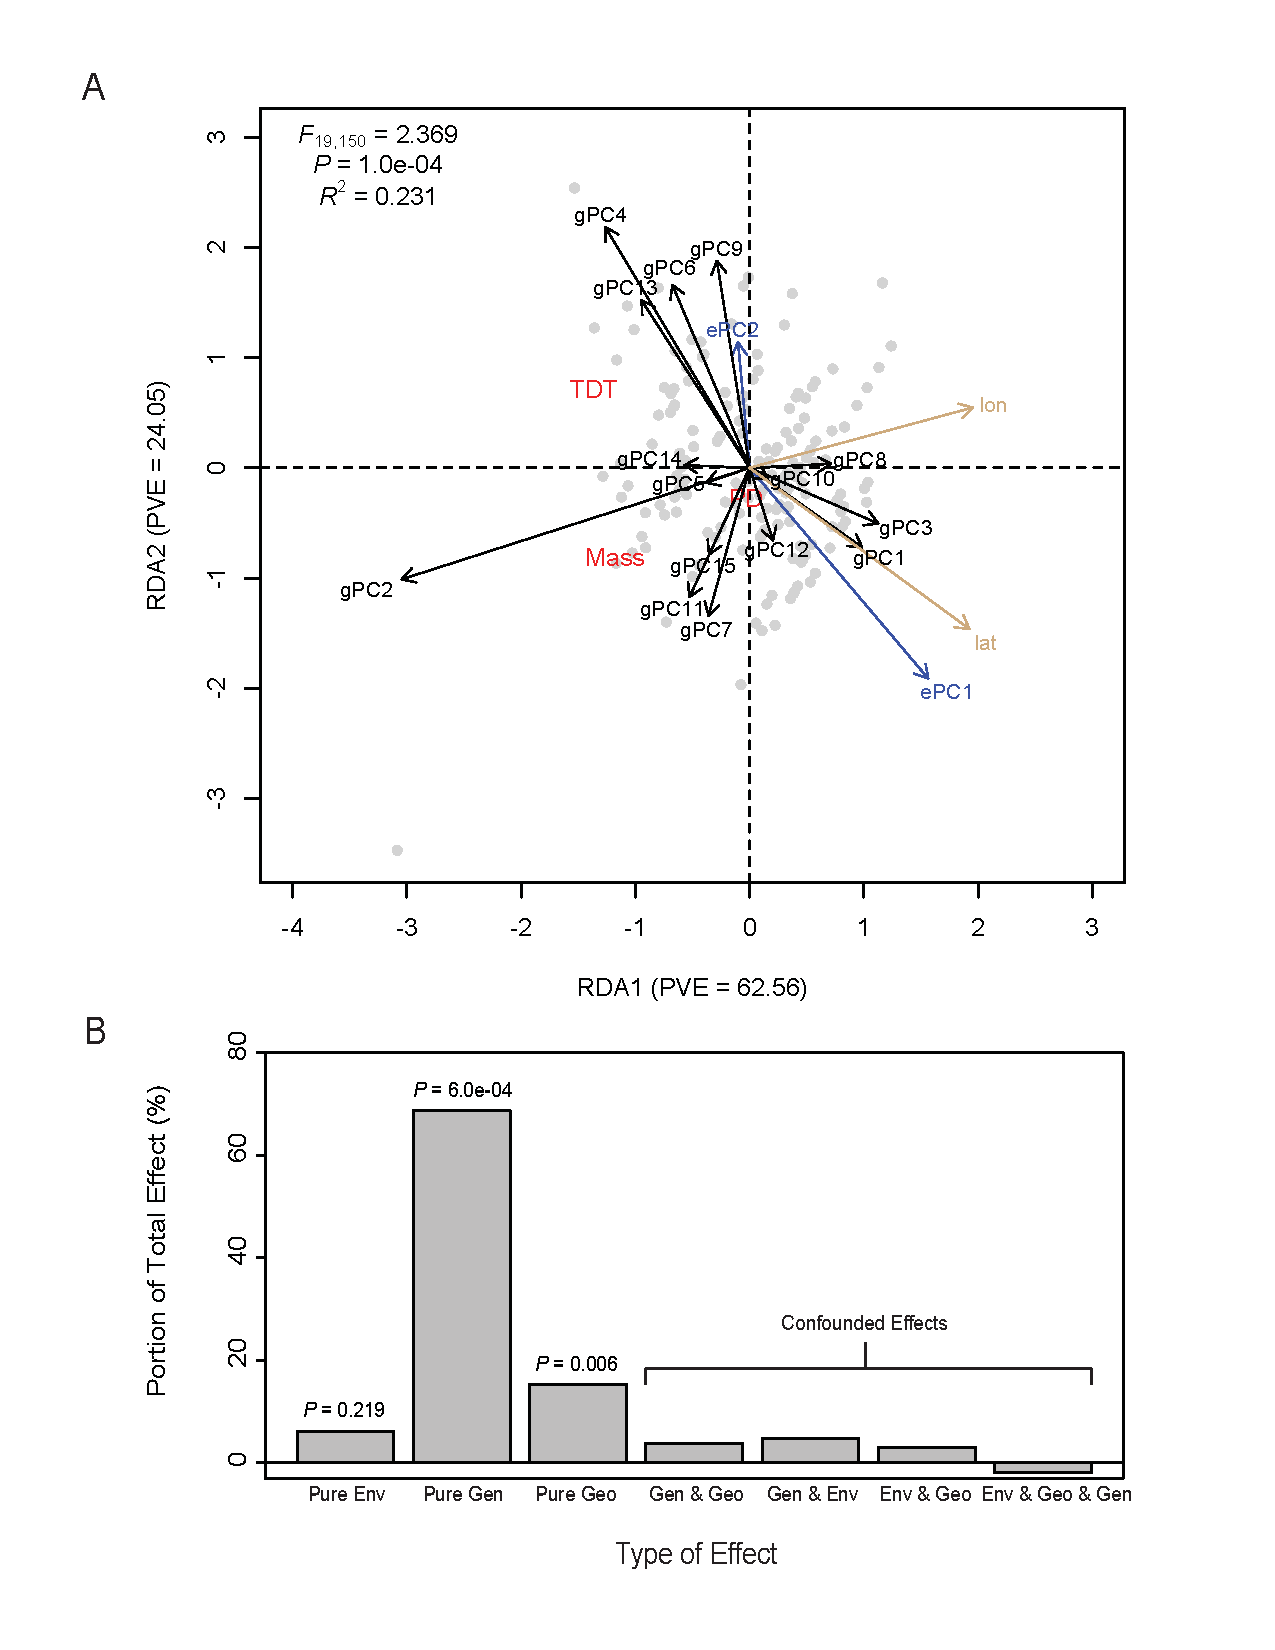
\includegraphics[width=0.9\textwidth]{rda_fig}
\caption{TODO}
\label{fig:rda}
\end{figure}

\clearpage

\section*{Tables}
TODO


\clearpage


\beginsupplement%

\section*{Supplementary Materials}
TODO

\subsection*{Supplementary Text}\label{ss:supp}

%pandoc --from=docx --to=latex gypsy_supplemental_stuff.docx -o
%gypsy_supplemental_stuff.tex --extract-media=.

\textbf{Table SX.} Summary of one-way Analysis of Variance (ANOVA)
models testing for an effect of population labels on phenotypic trait
values

\begin{longtable}[c]{@{}llllll@{}}
\toprule
Phenotype & \emph{df} & SS & MS & \emph{F} &
\emph{P}-value\tabularnewline
\midrule
\endhead
\textbf{Mass} & & & & &\tabularnewline
Population & 5 & 14.679 & 2.936 & 3.12 & 0.01021\tabularnewline
Residuals & 164 & 154.321 & 0.941 & &\tabularnewline
\textbf{PD} & & & & &\tabularnewline
Population & 5 & 9.474 & 1.895 & 1.948 & 0.08912\tabularnewline
Residuals & 164 & 159.526 & 0.973 & &\tabularnewline
\textbf{TDT} & & & & &\tabularnewline
Population & 5 & 34.307 & 6.861 & 8.3543 & 4.658e-07\tabularnewline
Residuals & 164 & 134.693 & 0.821 & &\tabularnewline
\bottomrule
\end{longtable}

\textbf{Table SX.} Summary of RDA and pRDA models used to partition the
total effect of genetics (Gen), environment (Env), and geography (Geo)
on the multivariate phenotypes (Phen) of 170 gypsy moths sampled from
six natural populations following Liu (1997)

\begin{longtable}[c]{@{}lllllll@{}}
\toprule
Model & \emph{F} & \emph{df\textsubscript{1}} &
\emph{df\textsubscript{2}} & \emph{P}-value &
\emph{R}\textsuperscript{2} &
\emph{R}\textsuperscript{2}\textsubscript{adj}\tabularnewline%
\midrule
\endhead%
Phen \textasciitilde{} Gen\textbar{} (Geo + Env) & 2.0626 & 15 & 150 &
0.0004 & 0.1587 & 0.0837\tabularnewline%
Phen \textasciitilde{} Geo + Env & 3.2070 & 4 & 165 & 0.0003 & 0.0721 &
0.0496\tabularnewline%
Phen \textasciitilde{} (Geo + Env)\textbar{}Gen & 2.7597 & 4 & 150 &
0.0042 & 0.0566 & 0.0396\tabularnewline%
Phen \textasciitilde{} Gen & 2.1655 & 15 & 154 & 0.0005 & 0.1742 &
0.0937\tabularnewline%
Phen \textasciitilde{} Geo\textbar{} (Gen + Env) & 3.4431 & 2 & 150 &
0.0055 & 0.0353 & 0.0279\tabularnewline%
Phen \textasciitilde{} Gen + Env & 2.1725 & 17 & 152 & 0.0001 & 0.1955 &
0.1055\tabularnewline%
Phen \textasciitilde{} (Gen + Env)\textbar{}Geo & 2.1078 & 17 & 150 &
0.0003 & 0.1838 & 0.0977\tabularnewline%
Phen \textasciitilde{} Geo & 4.1217 & 2 & 167 & 0.0006 & 0.0470 &
0.0356\tabularnewline%
Phen \textasciitilde{} Env\textbar{} (Geo + Gen) & 1.3837 & 2 & 150 &
0.2227 & 0.0142 & 0.0044\tabularnewline%
Phen \textasciitilde{} Geo + Gen & 2.4721 & 17 & 152 & 0.0001 & 0.2166 &
0.1290\tabularnewline%
Phen \textasciitilde{} (Geo + Gen)\textbar{}Geo & 2.3264 & 17 & 150 &
0.0003 & 0.2028 & 0.1170\tabularnewline%
Phen \textasciitilde{} Env & 2.4044 & 2 & 167 & 0.0352 & 0.0280 &
0.0163\tabularnewline%
\bottomrule
\end{longtable}


% \begin{figure}[ht]
% \centering
% \includegraphics[width=0.9\textwidth]{}
% \caption{TODO}
% \label{fig:rda}
% \end{figure}

\begin{figure}
\centering
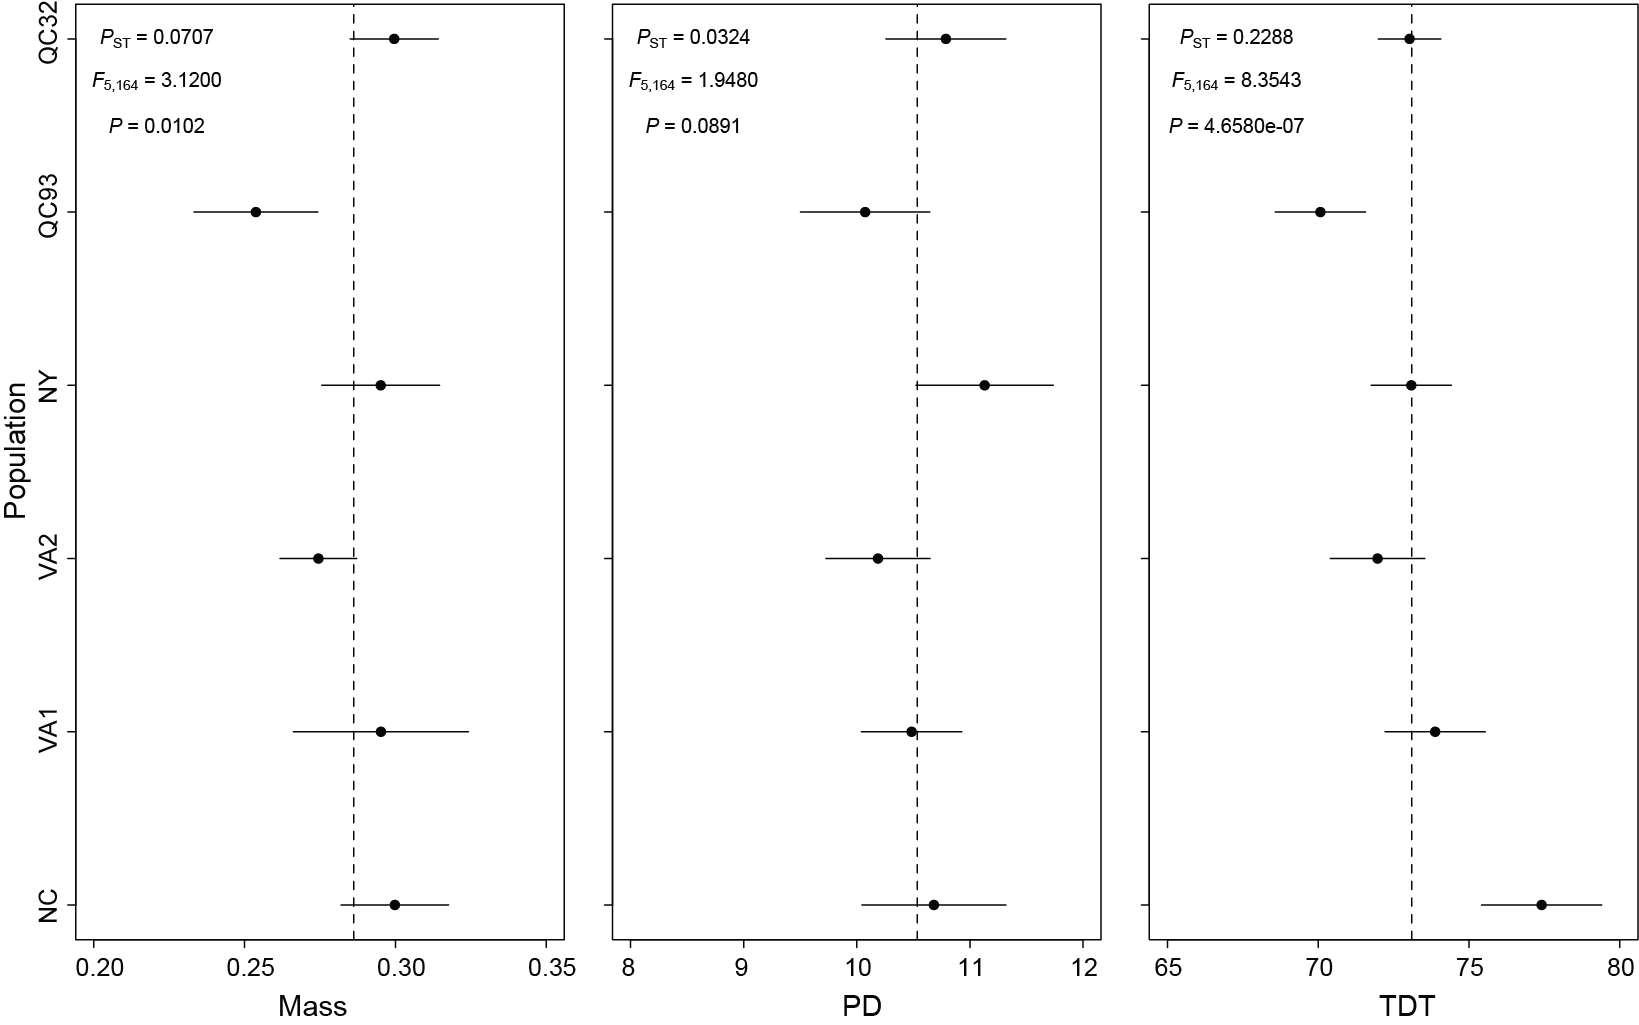
\includegraphics[width=0.9\textwidth]{media/image1.png}
\caption{Mean trait values and their 95\% confidence
intervals (±1.96 × s.e.m) by population for pupal mass (Mass), pupal
duration time (PD), and total development time (TDT). Vertical dashed
lines represent global means for each phenotypic trait.}
\label{fig:trait}
\end{figure}


\begin{figure}
\centering
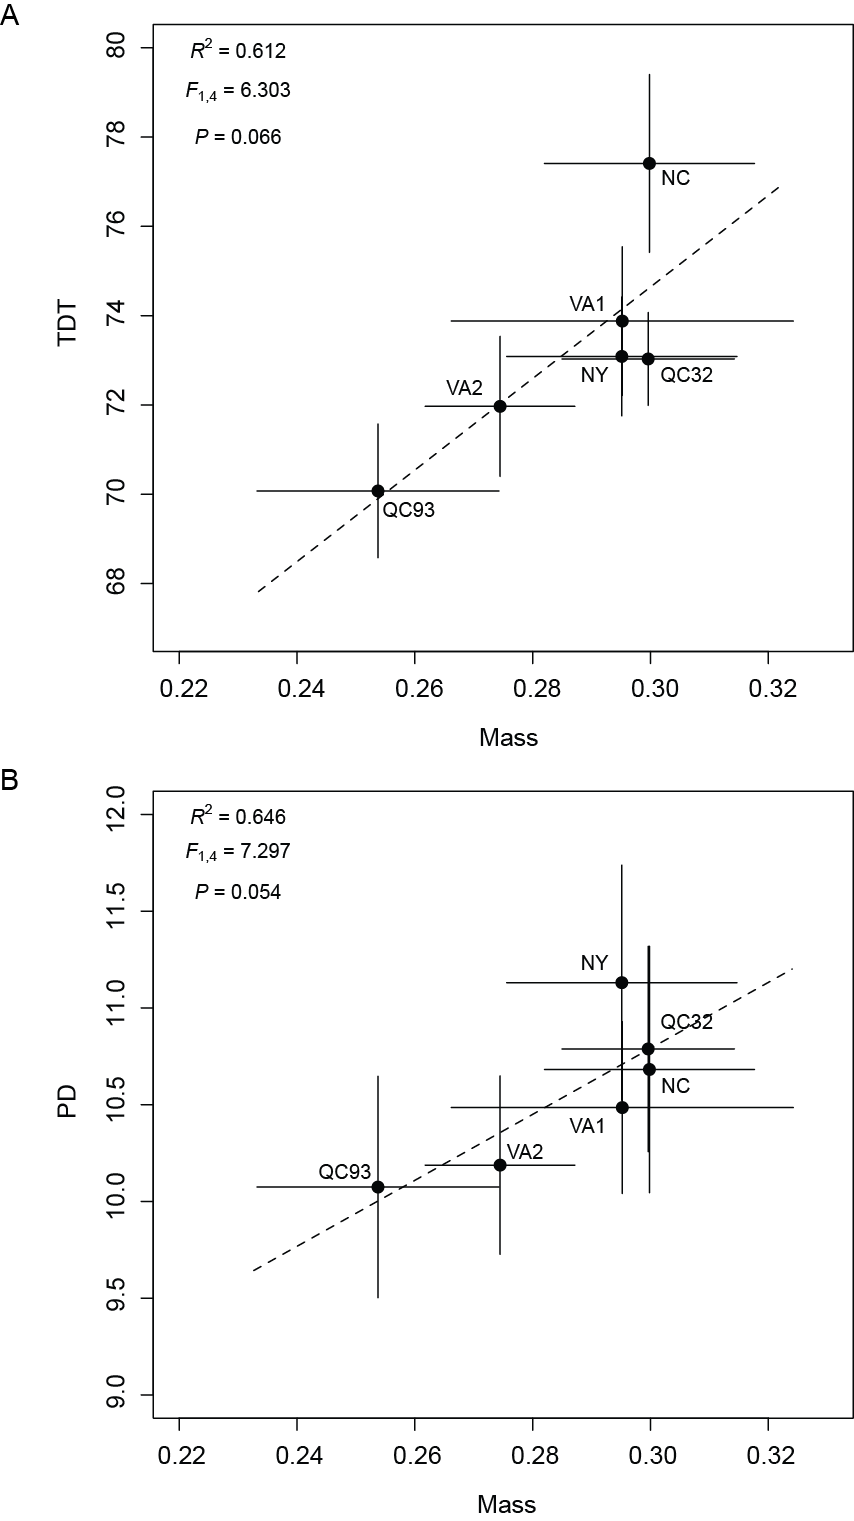
\includegraphics[width=0.6\textwidth]{media/image2.png}
\caption{Correlations among phenotypic trait means by
population that were marginally significant, (A) Pupal mass (Mass)
versus total development time (TDT), (B) Pupal mass (Mass) versus pupal
development time (PD). Statistics in the upper right corner were
generated using a linear model with pupal mass as the predictor of TDT
and PD.}
\label{fig:traitcorr}
\end{figure}


\subsection*{Supplementary Figures}\label{ss:sfig}

\subsection*{Supplementary Tables}\label{ss:stab}



\end{document}
